\unnumsec{Nombres complexes}


\subsection{Définition des nombres complexes}
Considérons la ligne des nombres réels
\begin{figure}[!htbp]
    \begin{center}
        \def\numberLineLastNumber{7}
        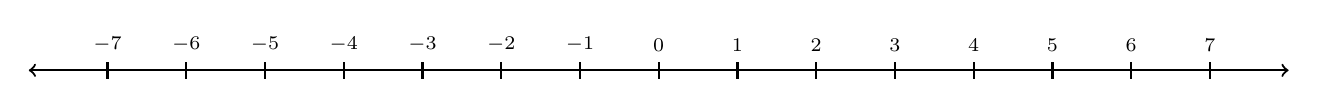
\begin{tikzpicture}
            \begin{scope}[thick,font=\scriptsize]

                \draw [<->] (-\numberLineLastNumber - 1,0) -- (\numberLineLastNumber + 1,0);

                \foreach \n in {-\numberLineLastNumber,...,\numberLineLastNumber}{%
                        \draw (\n,-3pt) -- (\n,3pt)   node [above] {$\n$};
                    }
            \end{scope}
        \end{tikzpicture}
    \end{center}
    \caption{La ligne des nombres réels}
\end{figure}
\begin{remark}
    Chaque nombre réel peut être représenté par un vecteur qui commence de 0 et qui a le nombre comme magnitude. L'angle du vecteur est encodé dans le signe du nombre, un nombre positif va avoir un vecteur d'un angle de 0 et un nombre négatif va avoir un vecteur d'un angle de $\pi$
\end{remark}

\begin{figure}[!htbp]
    \begin{center}
        \def\numberLineLastNumber{7}
        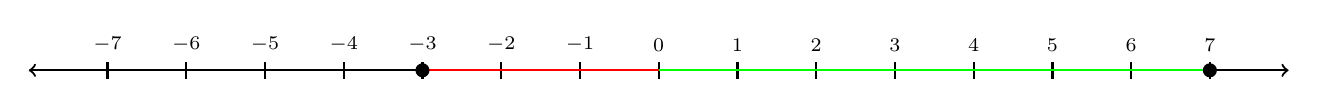
\begin{tikzpicture}
            \begin{scope}[thick,font=\scriptsize]

                \draw [<->] (-\numberLineLastNumber - 1,0) -- (\numberLineLastNumber + 1,0);

                \foreach \n in {-\numberLineLastNumber,...,\numberLineLastNumber}{%
                        \draw (\n,-3pt) -- (\n,3pt)   node [above] {$\n$};
                    }

                \draw [-, thick, color=red] (0,0) -- (-3,0);
                \draw [-, thick, color=green] (0,0) -- (7,0);
                \draw [color=black, fill=black] (-3,0) circle(0.075);
                \draw [color=black, fill=black] (7,0) circle(0.075);

            \end{scope}
        \end{tikzpicture}
    \end{center}
    \caption{Le vecteur des nombres -3 et 7 représenté sur la ligne des nombres réels}
\end{figure}
\begin{remark}
    Dans cette représentation, les vecteurs ont seulement des angles de 0 ou $\pi$. Pour que les vecteurs aillent des angles arbitraires, nous devons introduire un autre axe.
\end{remark}
\begin{definition}
    $i$ est l'unité imaginaire telle que $i^2 = -1$
\end{definition}
Comme dans le cas des nombres réels, il est possible de tracer une ligne des nombres imaginaires. Par convention, cette ligne est tracée perpendiculaire à la ligne des nombres réels. Ainsi, la ligne des nombres imaginaires est justement ce qu'il faut pour pouvoir représenter des vecteurs avec des angles arbitraires.
\begin{figure}[!htbp]
    \begin{center}
        \begin{tikzpicture}
            \begin{scope}[thick,font=\scriptsize]

                \draw [->] (-3.5,0) -- (4,0) node [above]  {Axe réel};
                \draw [->] (0,-3.5) -- (0,4) node [below right] {Axe imaginaire};

                \foreach \n in {-3,...,-1,1,2,...,3}{%
                        \draw (\n,-3pt) -- (\n,3pt)   node [above] {$\n$};
                        \draw (-3pt,\n) -- (3pt,\n)   node [right] {$\n i$};}

                \draw [thick, color=red] (0,0) -- (2,2);
                \draw [color=black, fill=black] (2,2) circle(0.05);
                \node [color=black] at (2,2.25) {$ 2+2i$};
            \end{scope}
        \end{tikzpicture}
    \end{center}
    \caption{Représentation du vecteur qui a une magnitude de $2\sqrt{2}$ et un angle de $\frac{\pi}{4}$}
    \label{complex_plane}
\end{figure}

\begin{definition}
    L'ensemble qui est représenté par la ligne des nombres réels et la ligne des nombres imaginaires est appelé les nombres complexes et est noté $\C$
\end{definition}

\subsection{Représentation des nombres complexes}
Considérons la figure suivante:
\begin{figure}[!htbp]
    \begin{center}
        \begin{tikzpicture}
            \begin{scope}[thick,font=\scriptsize]
                \coordinate (start) at (4,0);
                \coordinate (middle) at (0,0);
                \coordinate (end) at (2, 3);

                \draw [->] (-0.5,0) -- (4,0) node [above]  {Axe réel};
                \draw [->] (0,-0.5) -- (0,4) node [below right] {Axe imaginaire};

                \draw [thick, color=red] (0,0) -- (2,3);
                \node [color=black] at (0.88, 1.62) {$r$};
                \pic [draw, -, "$\theta$", angle eccentricity=1.5] {angle = start--middle--end};

                \draw [color=blue, fill=blue] (2,3) circle(0.05);
                \node [color=black] at (2,3.25) {$z \in \C$};

                \draw [thick, color=green] (0,0) -- (2, 0);
                \node [color=black] at (1, -0.25) {$x$};

                \draw [thick, color=green] (2,0) -- (2, 3);
                \node [color=black] at (2.25, 1.5) {$y$};

            \end{scope}
        \end{tikzpicture}
    \end{center}
    \caption{Représentation d'un nombre complexe}
\end{figure}

\begin{definition}
    $x$ est la partie réelle de $z$ et est notée $\Real{z}$
\end{definition}
\begin{definition}
    $y$ est la partie imaginaire de $z$ et est notée $\Ima{z}$
\end{definition}
\begin{definition}
    $r$ est le module de $z$ et est noté $|z|$
\end{definition}
\begin{lemma} On peut calculer le module de $z$ à partir de sa partie réelle et imaginaire avec
    \[|z| = r = \sqrt{x^2 + y^2}\]
\end{lemma}
\begin{definition}
    $\theta$ est l'argument de $z$ noté $\text{Arg}(z)$. Cet argument est unique et par convention est entre $-\pi$ et $\pi$, soit $-\pi < \text{Arg}(z) \leq \pi$.
\end{definition}
\begin{definition}
    L'argument non unique de $z$ est $\arg(z) = \text{Arg}(z) + 2\pi k, \ k \in \Z$
\end{definition}
\begin{lemma}
    On peut calculer l'argument de $z$ à partir de sa partie réelle et imaginaire avec
    \[\textup{Arg}(z) = \theta =
        \begin{cases}
            \arctan(\frac{y}{x})          & x > 0                                                  \\
            \arctan(\frac{y}{x}) - \pi    & x < 0                                                  \\
            \textup{sign}(y)\frac{\pi}{2} & x = 0, \ \textup{sign}(y) \ \textup{est la signe de y}
        \end{cases}\]
\end{lemma}
On peut remarquer qu'un nombre complexe est entièrement déterminé par sa partie réelle et imaginaire. On peut représenter un nombre complexe de trois formes différentes. Si on utilise seulement $x$ et $y$ pour représenter ces deux parties, on obtient la première forme d'un nombre complexe:
\begin{definition}
    La \underline{forme algébrique} (ou cartésienne) de $z$ est $z = x + iy, \ x, y \in \R$
\end{definition}
Si on utilise seulement $r$ et $\theta$ pour représenter la partie réelle et imaginaire, on obtient la deuxième forme d'un nombre complexe:
\begin{definition}
    La \underline{forme polaire} de $z$ est $z = r(\cos(\theta)+i\sin(\theta)), \ r, \theta \in \R$
\end{definition}
Il existe une troisième forme d'un nombre complexe. Cette forme utilise la formule d'Euler, qui est:
\begin{theorem}[Formule d'Euler]
    \[ e^{i\theta} = \cos{\theta} + i\sin{\theta} \]
\end{theorem}
En utilisant la formule d'Euler on obtient la forme exponentielle:
\begin{definition}
    La \underline{forme exponentielle} de $z$ est $z = re^{i\theta}, \ r, \theta \in \R$
\end{definition}
\begin{note}
    Les trois formes sont équivalentes, c-à-d $z = x + iy = r(\cos{\theta} + i\sin{\theta}) = re^{i\theta}$
\end{note}

\begingroup
\renewcommand{\arraystretch}{1.5}

\subsection{Le conjugué d'un nombre complexe}
\begin{definition}
    Le conjugé de $z = x + iy$ est noté $z^*$ ou $\bar{z}$ et est donné par $z^* = x - iy = \Real{z} - i\Ima{z}$
\end{definition}
\begin{remark}
    Le conjugué est involutif, c-à-d $\left(z^* \right)^* = z$
\end{remark}

\subsubsection{Propriétés du conjugué et du module}
Le conjugué et le module sont distributifs sur l'addition, la multiplication et la division.
\begin{center}
    \begin{tabular}{c@{\hskip 1in} c@{\hskip 1in} c}
        Addition                                   & Multiplication                          & Division                                                  \\
        $\left(z_1 + z_2\right)^* = z_1^* + z_2^*$ & $\left(z_1z_2\right)^* = z_1^{*} z_2^*$ & $\left( \frac{z_1}{z_2}\right)^{*} = \frac{z_1^*}{z_2^*}$ \\
        $\left|z_1 + z_2\right| = |z_1| + |z_2|$   & $\left|z_1z_2\right| = |z_1||z_2|$      & $\left| \frac{z_1}{z_2}\right| = \frac{|z_1|}{|z_2|}$
    \end{tabular}
\end{center}
Le conjugué et le module sont reliés par l'équation
\[
    zz^* = |z|^2
\]
\subsubsection{Propriétés de l'argument}
L'argument de $z$ a des propriétés semblables aux propriétés logarithmiques
\begin{center}
    \begin{tabular}{c@{\hskip 1in}c}
        Produit à somme                        & Quotient à différence                                       \\
        $\arg(z_1z_2) = \arg(z_1) + \arg(z_2)$ & $\arg\left( \frac{z_1}{z_2}\right) = \arg(z_1) - \arg(z_2)$
    \end{tabular}
\end{center}

\endgroup

\subsection{Racines entières}
\label{whole_roots}
Soit $z = re^{i\theta},\ n \in \N$. Alors $z$ à la racine de $n$ est donné par
\[
    \sqrt[n]{z} = \sqrt[n]{r} \left( e^{i \left( \frac{\theta + 2\pi k}{n} \right) } \right), \ k = 0, \dots, n - 1
\]
On peut aussi calculer les racines de $z$ de manière récursive. \\
Si $w$ est une racine de $z$, alors on a
\[
    w_k = \begin{cases}
        w_{k - 1}e^{ \frac{2\pi i}{n} }                    & k > 0 \\[0.5em]
        \sqrt[n]{r} \left( e^{i \frac{\theta}{n} } \right) & k = 0
    \end{cases}
\]
\begin{remark}
    Deux racines entières consécutives sont séparées par un angle de $\frac{2\pi}{n}$
\end{remark}

\subsection{Exponentielle  et logarithme}
Soit $z \in \C$, alors l'exponentielle de $z$ noté $e^z$ est
\[
    e^z = e^x e^{iy} = e^x (\cos(y) + i\sin(y))
\]
De plus, le logarithme de $z$ noté $\ln{z}$ ou $\log{z}$ est
\begin{align*}
    \ln(z) = \log(z) & = \ln|z| + i(\theta + 2\pi k), \ k \in \Z        \\
                     & = \ln|z| + i(\text{Arg}(z) + 2\pi k), \ k \in \Z \\
                     & = \ln|z| + i\arg(z)                              \\
\end{align*}

\subsection{Puissances complexes}
Soient $z, w \in \C$ où $w = x + iy$, alors $z$ à la $w$ est donnée par
\[
    z^w = |z|^{x} e^{-y\text{Arg}(z)} e^{2\pi yk} e^{ i \left(x\arg(z) + y\ln|z|\right) }, \; k \in \Z
\]
Il y a deux cas qui déterminent le nombre de valeurs de $z^w$
\begin{enumerate}
    \item Si $y \neq 0$ alors $z^w$ prend une infinité de valeurs distinctes, puisque $e^{2\pi yk} \neq 1 \ \forall \ k \in \Z$
    \item Si $y = 0$ alors le nombre de valeurs dépend de $x$
          \begin{enumerate}
              \item Si $x \in \Q$, alors c'est le cas des racines entières [\ref{whole_roots}]
              \item Si $x \in \R \backslash \Q$, alors $z^w$ prend une infinité de valeurs avec une partie imaginaires qui varie et une partie réelle qui reste fixe.
          \end{enumerate}
\end{enumerate}
\begin{remark}
    Dans ce dernier cas, si $z, w \in \R$ alors, par convention, on prend $k = 0$ pour que $z^w \in \R$.
\end{remark}

\subsection{Théorème fondamental de l'algèbre}
Considérons le polynôme complexe $p(x)$ de degré $n \in \N$. Il est possible d'écrire $p(x)$ sous sa forme générale, qui est:
\[
    p(x) = a_n x^n + a_{n-1} x^{n-1} + \dots + a_1 x + a_0, \; a_j \in \C, \; a_n \neq 0
\]
\begin{definition}
    Les racines d'un polynôme complexe sont des valeurs complexes $t \in \C$ telles que $p(t) = 0$
\end{definition}
\begin{lemma}
    Il est possible d'écrire $p(x)$ en terme de ses $m$ racines, $\{t_1, t_2, \dots ,t_m\}$, c-à-d
    \[ p(x) = a_n(x - t_1)^{k_1} (x - t_2)^{k_2} \dots (x - t_m)^{k_m} \]
    où $k_j$ est la multiplicité de la racine $t_j$
\end{lemma}
\begin{lemma}
    \label{sum_multiplicity}
    La somme des $m$ multiplicités donne $n$, c-à-d $k_1 + k_2 + \dots + k_m = n$
\end{lemma}
D'après le lemme \ref{sum_multiplicity} nous pouvons formuler le théorème suivant:
\begin{theorem}[Théorème fondamental de l'algèbre]
    \label{theorem_fondamental_algebra}
    $p(x)$ a exactement $n$ racines complexes en comptant les multiplicités.
\end{theorem}